\pdfminorversion=4
\documentclass[aspectratio=169]{beamer}

\mode<presentation>
{
  \usetheme{default}
  \usecolortheme{default}
  \usefonttheme{default}
  \setbeamertemplate{navigation symbols}{}
  \setbeamertemplate{caption}[numbered]
  \setbeamertemplate{footline}[frame number]  % or "page number"
  \setbeamercolor{frametitle}{fg=white}
  \setbeamercolor{footline}{fg=black}
}

\usepackage[english]{babel}
\usepackage[utf8x]{inputenc}
\usepackage{tikz}
\usepackage{courier}
\usepackage{array}
\usepackage{bold-extra}
\usepackage{minted}
\usepackage[thicklines]{cancel}
\usepackage{fancyvrb}

\xdefinecolor{dianablue}{rgb}{0.18,0.24,0.31}
\xdefinecolor{darkblue}{rgb}{0.1,0.1,0.7}
\xdefinecolor{darkgreen}{rgb}{0,0.5,0}
\xdefinecolor{darkgrey}{rgb}{0.35,0.35,0.35}
\xdefinecolor{darkorange}{rgb}{0.8,0.5,0}
\xdefinecolor{darkred}{rgb}{0.7,0,0}
\definecolor{darkgreen}{rgb}{0,0.6,0}
\definecolor{mauve}{rgb}{0.58,0,0.82}

\title[2019-07-10-awkward-plans]{Awkward plans}
\author{Jim Pivarski}
\institute{Princeton University -- IRIS-HEP}
\date{July 10, 2019}

\usetikzlibrary{shapes.callouts}

\begin{document}

\logo{\pgfputat{\pgfxy(0.11, 7.4)}{\pgfbox[right,base]{\tikz{\filldraw[fill=dianablue, draw=none] (0 cm, 0 cm) rectangle (50 cm, 1 cm);}\mbox{\hspace{-8 cm}
\includegraphics[height=1 cm]{princeton-logo-long.png}\hspace{0.1 cm}\raisebox{0.1 cm}{
\includegraphics[height=0.8 cm]{iris-hep-logo-long.png}}\hspace{0.1 cm}}}}}

\begin{frame}
  \titlepage
\end{frame}

\logo{\pgfputat{\pgfxy(0.11, 7.4)}{\pgfbox[right,base]{\tikz{\filldraw[fill=dianablue, draw=none] (0 cm, 0 cm) rectangle (50 cm, 1 cm);}\mbox{\hspace{-8 cm}
\includegraphics[height=1 cm]{princeton-logo.png}\hspace{0.1 cm}\raisebox{0.1 cm}{
\includegraphics[height=0.8 cm]{iris-hep-logo.png}}\hspace{0.1 cm}}}}}

% Uncomment these lines for an automatically generated outline.
%\begin{frame}{Outline}
%  \tableofcontents
%\end{frame}

% START START START START START START START START START START START START START

\begin{frame}{Context}
\large
\vspace{0.25 cm}
Awkward-array is the end of a long chain of ideas about columnar analysis:

\vspace{0.25 cm}
\mbox{\hspace{-1.7 cm}\begin{minipage}{1.2\linewidth}
\begin{description}\setlength{\itemsep}{0.1 cm}
  \item[2016] \textcolor{darkblue}{Femtocode} was originally envisioned as a combined language, columnar processor, and distributed processing system: a full-service package for physics.
  \item[$\bullet$] To be more realistic, I separated the language and columnar processing from the distributed processing, leaving the latter to others.
  \item[2017] \textcolor{darkblue}{Shredtypes} $\to$ \textcolor{darkblue}{Quiver} (for Arrow) $\to$ \textcolor{darkblue}{OAMap} were iterations on expressing an abstract type system with an internal columnar representation.
  \item[$\bullet$] \textcolor{darkblue}{Uproot 2} had a ``minimal columnar data type'': a {\tt JaggedArray} class.
  \item[2018] Users found {\tt JaggedArrays} useful despite the fact that it doesn't hide the columnar representation (this was a surprise to me).
  \item[$\bullet$] \textcolor{darkblue}{Awkward-array} built the abstract type system to columnar representation in the other direction: bottom-up, from physical arrays to abstract types.
  \item[2019] \textcolor{darkblue}{Awkward-array} is the first in this series to be widely used; I'm getting a lot of feedback from Coffea and \textcolor{darkblue}{uproot 3} users.
\end{description}
\end{minipage}}
\end{frame}

\begin{frame}{Up to now: one specification, many implementations}
\large
\vspace{0.5 cm}

Four of my ``ongoing projects'' are different implementations of awkward, all to adhere to the {\tt specification.adoc} (which is now out of date).

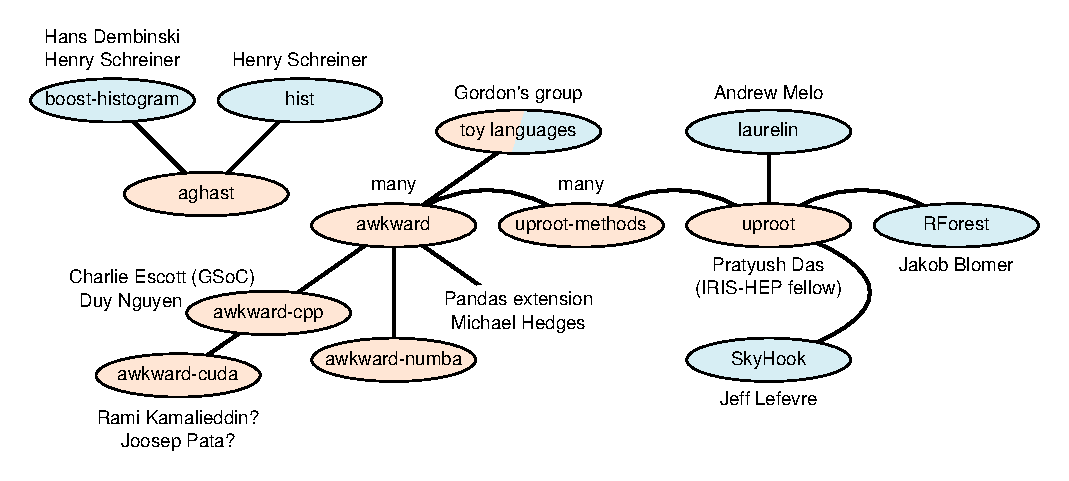
\includegraphics[width=\linewidth]{projects.pdf}
\end{frame}

\begin{frame}{Just finished a homogenization/documentation campaign}
\vspace{0.25 cm}
\begin{columns}
\column{0.35\linewidth}
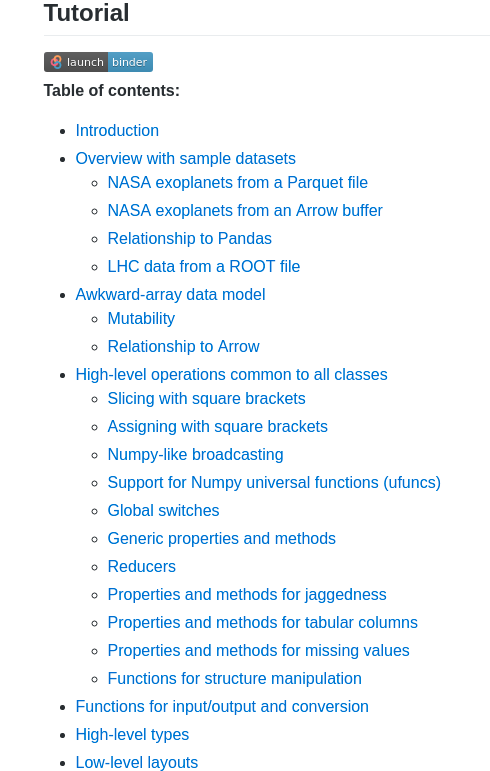
\includegraphics[width=\linewidth]{awkward-documentation.png}

\column{0.55\linewidth}
``Homogenization'' because a common user complaint is that methods defined on one class (e.g. {\tt JaggedArray}) don't work on another class (e.g. {\tt MaskedArray} of {\tt JaggedArray}).

\vspace{0.5 cm}
While documenting (100 pages of examples), I ensured that a suite of ``high-level'' methods does something meaningful on every array class.
\end{columns}
\end{frame}

\begin{frame}{Problems}
\large
\vspace{0.5 cm}
\begin{enumerate}\setlength{\itemsep}{0.2 cm}
\item Writing the same method on 14 classes $\times$ 4 implementations is a problem for developer FTEs now and maintainance later.

\textcolor{gray}{(Remember, I haven't touched awkward-numba since February!)}

\item Users need a better separation between high-level and low-level.

\begin{itemize}\normalsize\setlength{\itemsep}{0.2 cm}
\item Structural classes, such as {\tt ChunkedArray} of {\tt VirtualArrays} of {\tt X} to make array {\tt X} lazy-loading, should be hidden.

\item Named methods, like \mintinline{python}{x.cross(y)} meaning ``cross-join,'' compete for the same namespace with column names and domain-specific methods, like \mintinline{python}{x.cross(y)} meaning ``3-D cross product.''
\end{itemize}

\item Too many features are opt-in. Numba integration will fail and Pandas integration will have a subtle performance bug if the user doesn't \mintinline{python}{import awkward.numba} and \mintinline{python}{import awkward.pandas} first.

\end{enumerate}
\end{frame}

\begin{frame}{Solution to \#1: implement at most twice}
\vspace{0.1 cm}

\begin{columns}
\column{0.55\linewidth}
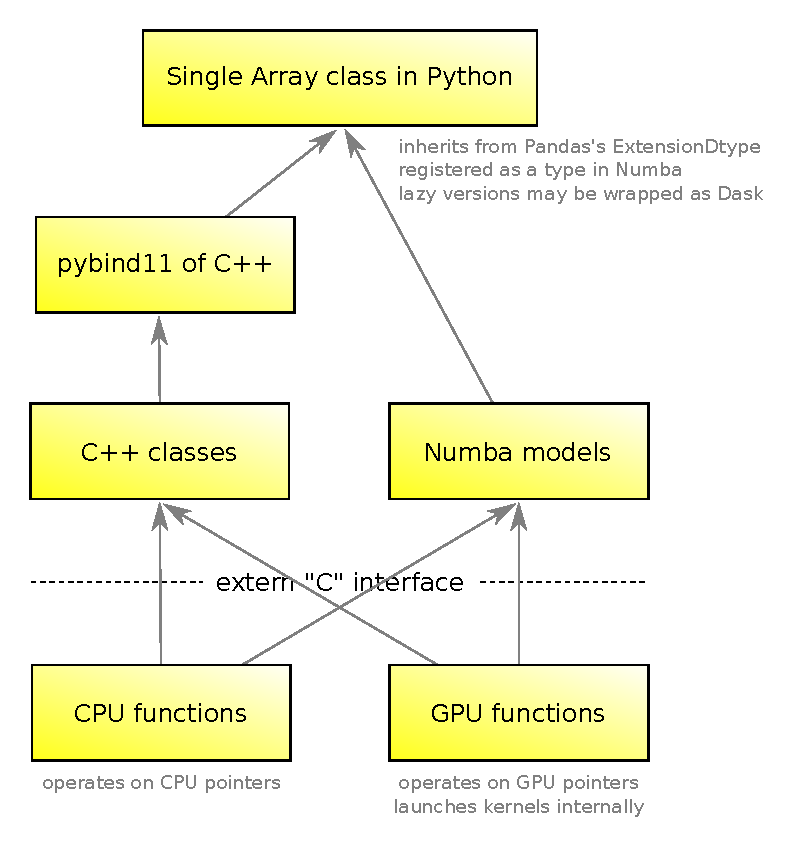
\includegraphics[width=\linewidth]{awkward-1-0-layers.pdf}

\column{0.5\linewidth}
Put all CPU implementations behind a stateless \mintinline{c++}{extern "C"} interface.

\begin{itemize}
\item C++ classes (e.g. {\tt JaggedArray}) provide structure and ownership rules.
\item Numba (e.g. {\tt JaggedArrayModel}) extensions associate Python classes in \mintinline{python}{@numba.jit} functions with the same implementations.
\item Structure classes mirrored between C++ and Python by pybind11.
\item Structure classes hidden inside {\tt Array}.
\end{itemize}

Maybe later write \mintinline{c++}{extern "C"} functions for GPU as well.
\end{columns}
\end{frame}

\begin{frame}[fragile]{Solution to \#2a: separation between high-level and low-level}
\large
\vspace{0.5 cm}

Single {\tt Array} class with a high-level type; narrow access to underlying structure.

\small
\vspace{0.2 cm}
\mintinline{python}{>>> myarray}

\vspace{0.1 cm}
{\tt <Array [[1.1, 2.2, 3.3], [], [4.4, 5.5]] at 0x7fce7170bcf8>}

\vspace{0.2 cm}
\mintinline{python}{>>> print(awkward.arraytype(array))   # datashape.readthedocs.io}

\vspace{0.1 cm}
{\tt 3 * var * float64}

\vspace{0.2 cm}
\mintinline{python}{>>> array.struct}

\vspace{0.1 cm}
{\tt JaggedArray([3, 99, 0], [5, 99, 3], [4.4, 5.5, 1.1, 2.2, 3.3])}

\large
\vspace{0.3 cm}
The user only finds out that it is a {\tt JaggedArray}, and not a lazy {\tt JaggedArray}, by digging into the structure classes provided by pybind11.

\vspace{0.3 cm}
This also hides the \mintinline{python}{starts=[3, 99, 0]} and \mintinline{python}{stops=[5, 99, 3]}.
\end{frame}

\begin{frame}[fragile]{Solution to \#2b}
\large
\vspace{0.5 cm}

It would be easier to implement and a cleaner API to put structure-manipulation operations in free-standing functions like

\small
\begin{minted}{python}
awkward.cross([x, y, z])       # size of output known at the beginning
\end{minted}

\large
rather than

\small
\begin{minted}{python}
x.cross(y).cross(z)            # have to make intermediate arrays
\end{minted}

\large
\vspace{0.25 cm}
Apart from a single \textcolor{darkgreen}{\mintinline{python}{struct}} attribute and unnamed magic like \mintinline{python}{__add__}, \textcolor{blue}{\mintinline{python}{__array_ufunc__}}, etc., the {\tt Array} class can be kept clear for columns and domain-specific methods:

\small
\begin{minted}{python}
mydata.btag                    # field names as attributes
lorentzVectors.boost(others)   # physics methods
vector3Ds.cross(others)        # reduced ambiguity
\end{minted}

\large
In short, everything after the dot would be physics.
\end{frame}

\begin{frame}{Solution to \#3}
\large
\vspace{0.5 cm}

Originally, I didn't want to automatically register Numba types and automatically make awkward arrays descend Pandas's {\tt ExtensionDtype} because importing these libraries would add to the startup time, even if not used.

\begin{center}
\renewcommand{\arraystretch}{1.5}
\begin{tabular}{l c c c}
& slow computer & medium computer & fast computer \\
\mintinline{python}{import pandas} & 1.5 sec & 0.35 sec & 0.25 sec \\
\mintinline{python}{import numba} & 1.0 sec & 0.35 sec & 0.20 sec \\
\textcolor{blue}{\texttt{\textbf{pandas}}} and \textcolor{blue}{\texttt{\textbf{numpy}}} & 2.0 sec & 0.60 sec & 0.35 sec \\
\end{tabular}
\end{center}

\vspace{0.5 cm}
``Slow computer'' is 1.1 GHz, ``medium'' is 2.6 GHz. Most users will be fine.
\end{frame}

\begin{frame}{Drawbacks of this plan}
\vspace{0.25 cm}
\Large
\begin{itemize}
\item The original Numpy-based implementation and partial Numba-based one will have to be scrapped in favor of C++.

\uncover<2->{\textcolor{mauve}{It served us well. The feedback we got from getting something in front of users quickly was invaluable.}}

\item A major change in API, even a good one, will require roll-out: awkward 0.x $\to$ awkward 1.0.

\uncover<2->{\textcolor{mauve}{Since we envisioned multiple awkward implementations, uproot already has hooks for switching between alternatives.}}

\item After Charle Escott's GSoC ends, I'm the only developer.

\uncover<2->{\textcolor{mauve}{It's my time to learn C++11.  {\tt :)}}}

\item I estimate about 6 months for this transition.

\uncover<2->{\textcolor{mauve}{We already know it has a userbase.}}
\end{itemize}
\end{frame}

\begin{frame}{Not-originally-intended advantage}
\Large
\vspace{0.5 cm}
By putting the {\it primary} implementation in C++, awkward-array could be directly used by C++ projects.

\large
\vspace{0.25 cm}
\begin{itemize}\setlength{\itemsep}{0.25 cm}
\item Easier to emit awkward arrays from ATHENA/CMSSW: e.g.\ for ServiceX.
\item Could become a standard way to wrap C++ libraries for Pythonic analysis: e.g.\ {\tt JaggedArray} of 4-vectors $\to$ FastJet $\to$ {\tt JaggedArray} of jets.
\item Actually write production code with awkward-arrays, to transparently replace CPUs with GPUs? (Giuseppe Cerati has been looking into this.)
\end{itemize}

\end{frame}

\begin{frame}{My projected timeline}
\large
\vspace{0.5 cm}
\begin{description}\setlength{\itemsep}{0.2 cm}
\item[July:] two more tutorials: CoDaS-HEP and DPF (a total of 7 this year!)
\item[August:] Charlie's GSoC project finishes: learn as much as we can about pybind11's strengths and weaknesses
\item[August:] I finish the prototype SQL-for-events toy language
\item[September:] Strange Loop and working on fundamentals of awkward 1.0
\item[October:] Still working on awkward 1.0 and maybe go to PyHEP
\item[November:] CHEP and should be getting usable prototypes of awkward 1.0 to Coffea for testing
\item[December:] Should be transitioning PyPI packages \textcolor{darkgreen}{awkward0} and \textcolor{darkgreen}{awkward}
\end{description}

\begin{center}
\textcolor{gray}{--- --- --- then it's the year 2020 --- --- ---}
\end{center}
\end{frame}

\end{document}
